\section{Concept}

\subsection{Neural Network}

For the neural network we base the architecture of our network on the well known \emph{LeNet} architecture from \cite{LeCun:1998aa} is chosen due to its simplicity and ease to implement. Additionally the performance is improved by using modern, established techniques like batch normalization \cite{Ioffe:2015aa} and dropout \cite{Srivastava:2014aa} layers. 
The training of network is done using PyTorch \cite{Paszke:2019aa} on a regular PC and the trained network parameters are then used to create a hardware VHDL model of the network. An overview of the structure can be seen in Figure~\ref{fig:network-concept}. For verification all neural network operations are checked in separate programmed programs for correctness. See the Section~\ref{subsec:nntraining} for details how the network is implemented in Software.
An excellent overview in deep learning can be found in \cite{Schmidhuber:2015aa}.
To train and test the network we chose the MNIST dataset \cite{LeCun:1998ab}. It consists of 50.000 training images and 10.000 test images of handwritten digits, where each is 28-by-28 pixel.


\begin{figure}[htbp]
	\noindent\resizebox{\textwidth}{!}{
	\begin{tikzpicture}
		%\draw[use as bounding box, transparent] (-1.8,-1.8) rectangle (17.2, 3.2);

		% Define the macro.
		% 1st argument: Height and width of the layer rectangle slice.
		% 2nd argument: Depth of the layer slice
		% 3rd argument: X Offset --> use it to offset layers from previously drawn layers.
		% 4th argument: Options for filldraw.
		% 5th argument: Text to be placed below this layer.
		% 6th argument: Y Offset --> Use it when an output needs to be fed to multiple layers that are on the same X offset.

		\newcommand{\networkLayer}[6]{
			\def\a{#1} % Used to distinguish input resolution for current layer.
			\def\b{0.02}
			\def\c{#2} % Width of the cube to distinguish number of input channels for current layer.
			\def\t{#3} % X offset for current layer.
			\def\d{#4} % Y offset for current layer.

			% Draw the layer body.
			\draw[line width=0.3mm](\c+\t,0,\d) -- (\c+\t,\a,\d) -- (\t,\a,\d);                                                      % back plane
			\draw[line width=0.3mm](\t,0,\a+\d) -- (\c+\t,0,\a+\d) node[midway,below] {#6} -- (\c+\t,\a,\a+\d) -- (\t,\a,\a+\d) -- (\t,0,\a+\d); % front plane
			\draw[line width=0.3mm](\c+\t,0,\d) -- (\c+\t,0,\a+\d);
			\draw[line width=0.3mm](\c+\t,\a,\d) -- (\c+\t,\a,\a+\d);
			\draw[line width=0.3mm](\t,\a,\d) -- (\t,\a,\a+\d);

			% Recolor visible surfaces
			\filldraw[#5] (\t+\b,\b,\a+\d) -- (\c+\t-\b,\b,\a+\d) -- (\c+\t-\b,\a-\b,\a+\d) -- (\t+\b,\a-\b,\a+\d) -- (\t+\b,\b,\a+\d); % front plane
			\filldraw[#5] (\t+\b,\a,\a-\b+\d) -- (\c+\t-\b,\a,\a-\b+\d) -- (\c+\t-\b,\a,\b+\d) -- (\t+\b,\a,\b+\d);

			% Colored slice.
			\ifthenelse {\equal{#5} {}}
			{} % Do not draw colored slice if #4 is blank.
			{\filldraw[#5] (\c+\t,\b,\a-\b+\d) -- (\c+\t,\b,\b+\d) -- (\c+\t,\a-\b,\b+\d) -- (\c+\t,\a-\b,\a-\b+\d);} % Else, draw a colored slice.
		}

		% INPUT
		\node[] (input image) at (-3.75,0.5) {
\includegraphics[height=30mm]{img/mnist/mnist_input_5_28}};
		\networkLayer{3.0}{0.03}{-0.5}{0.0}{color=gray!80}{}

		% ENCODER
		\networkLayer{3.0}{0.1}{0.0}{0.0}{color=white}{conv}    % S1
		%\networkLayer{3.0}{0.1}{0.2}{0.0}{color=white}{}        % S2
		\networkLayer{2.5}{0.2}{0.6}{0.0}{color=white}{conv}    % S1
		\networkLayer{2.5}{0.2}{0.9}{0.0}{color=white}{}        % S2
		\networkLayer{2.0}{0.4}{1.3}{0.0}{color=white}{conv}    % S1
		\networkLayer{2.0}{0.4}{1.8}{0.0}{color=white}{}        % S2
		\networkLayer{1.5}{0.8}{2.3}{0.0}{color=white}{conv}    % S1
		\networkLayer{1.5}{0.8}{3.2}{0.0}{color=white}{}        % S2
		\networkLayer{1.0}{1.5}{4.1}{0.0}{color=white}{conv}    % S1
		\networkLayer{1.0}{1.5}{5.7}{0.0}{color=white}{}        % S2

		% DECODER
%		\networkLayer{1.0}{1.5}{7.7} {0.0}{color=white}{deconv} % S1
%		\networkLayer{1.0}{1.5}{9.3} {0.0}{color=white}{}       % S2
%		\networkLayer{1.5}{0.8}{11.2}{0.0}{color=white}{deconv} % S1
%		\networkLayer{1.5}{0.8}{12.1}{0.0}{color=white}{}       % S2
%		\networkLayer{2.0}{0.4}{13.3}{0.0}{color=white}{}       % S1
%		\networkLayer{2.0}{0.4}{13.8}{0.0}{color=white}{}       % S2
%		\networkLayer{2.5}{0.2}{14.8}{0.0}{color=white}{}       % S1
%		\networkLayer{2.5}{0.2}{15.1}{0.0}{color=white}{}       % S2
%		\networkLayer{3.0}{0.1}{15.8}{0.0}{color=white}{}       % S1
%		\networkLayer{3.0}{0.1}{16}  {0.0}{color=white}{}       % S2

		% OUTPUT
%		\networkLayer{3.0}{0.05}{17}{0.0}{color=red!40}{}          % Pixelwise segmentation with classes.
%		\node[] (output image) at (18,0.5) {\includegraphics[height=30mm]{vermeer.jpg}};
%

	\end{tikzpicture}
	}
	\caption{Example CNN.}
	\label{fig:network-concept}
\end{figure}

\begin{figure}
	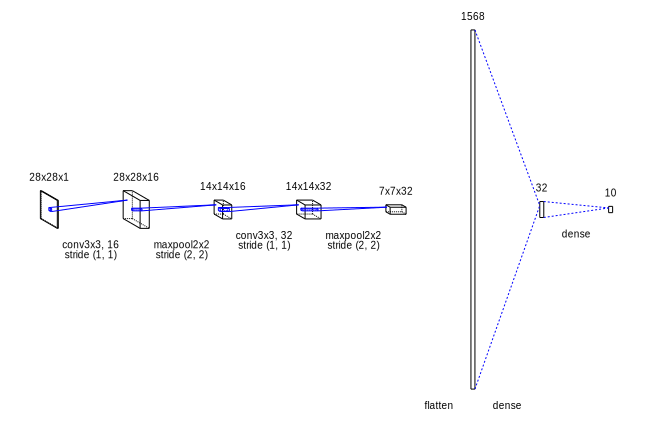
\includegraphics[width=0.8\textwidth]{../../net/images/network}
	\caption{Network overview}
	\label{fig:network-structure}
\end{figure}

\subsection{Hardware Concept}
\begin{figure}[h]
	\centering
	\includesvg[width=\textwidth]{img/inkscape/NN-concept.svg}
	\caption[Top-Level concept.]{Top-Level concept}
	\label{FIG:concept}
\end{figure}
\todo{Maybe add an additional Input Layer which is responsible to communicate with the DMA and converts the data from 32 bit to 8 bit and sends it to the memory controller}
\noindent
Figure \ref{FIG:concept} shows the Concept of implementing an FPGA-based hardware accelerator for handwritten digit recognition. It shows that the main components of the concepts are a Zedboard in combination with a remote PC or server. The handwritten digit recognition is performed by the Zedboard while the remote PC is used for training the network, for sending the image data to the Zedboard and for receiving the computed results.  The Zedboard includes a Zynq-7000 FPGA and provides various interfaces. \\
The neural network is implemented in the programmable logic part of the Zynq-7000. It is pre-trained using the remote PC, therefore only the inference of the neural network is implemented in hardware. \\
In order to train the network with the same bit resolution as implemented in the hardware, a software counterpart of the hardware is implemented in a PC using python. 
Based on the weights calculated by the python script a bitstream for the hardware is generated. This brings the benefit that for the convolutional layer constant multiplier can be used, since the weights of convolutional layer kernels are constant. For the dense layer it is not possible to implement the weights in a constant multiplier because in a dense layer each connection of a neuron requires a different weight, which would result in a huge amount of required constant multipliers. Therefore the weights for the dense layer have to be stored in a ROM inside the FPGA.   \\
